\chapter[Aplicaciones]{Aplicaciones de la Seguridad Informática}

\epigraph{\textit{''Las organizaciones gastan millones de dólares en firewalls y dispositivos de seguridad, pero tiran el dinero porque ninguna de estas medidas cubre el eslabón más débil de la cadena de seguridad: la gente que usa y administra los ordenadores''}}{--- Kevin Mitnick}

Con el objetivo de garantizar todos esos servicios mencionados en el capítulo anterior, se han desarrollado una gran cantidad de áreas dentro de la propia seguridad informática, que permiten cumplir con estos objetivos.

Las áreas de investigación y los campos de trabajo dentro de la seguridad informática avanzan a un ritmo acelerado debido al propio avance de la informática. El desarrollo de áreas como los smartphones o el Internet of Things (IoT) hace necesario nuevas técnicas que permitan garantizar la seguridad de la información a todos los niveles. Áreas como el ransomware, los wearables, los automóviles o el ciberespionaje son algunas en las que más hincapié se está haciendo en los últimos años \cite{mcafee-predictions}.

Teniendo eso en cuenta, durante este capitulo se describirán diferentes tipos de amenazas, tras lo cual se elaborará un análisis en mayor profundidad de las principales áreas que preocupan en el momento actual a la seguridad informática, que son los smartphones, el Internet of Things y el Cloud Computing.

%------------------------------------------------------------------------------

\section{Malware}

La seguridad informática siempre se ha relacionado con el concepto de virus informático. Si bien uno de los objetivos de la seguridad informática es evitar que este tipo de software consiga acceder a información o dañar sistemas, los virus informáticos no son la única manera que existe para comprometer la seguridad de la información. Sin embargo, el campo de la seguridad informática se desarrolla después de que surgieran estas primeras piezas de malware. Es debido al surgimiento de estas que se comprende la necesidad de desarrollar toda una serie de técnicas para garantizar la seguridad de la información almacenada y procesada en estos sistemas.

El concepto de malware es relativamente novedoso. El origen de programas capaces de replicarse y distribuirse se remonta hacia 1949, cuando el propio Von Neumann expuso \emph{La Teoría y Organización de Autómatas Complejos} \cite{von-neumann}, en la cual habla sobre pequeños autómatas capaces de replicarse por sí solos. Dos décadas después, concretamente en 1971, nace el denominado como primer virus informático de la historia, llamado \emph{Creeper} \cite{creeper} (enredadera en inglés).  Dicho virus no se puede considerar malware como tal ya que no causaba daño a los sistemas en los que se replicaba, simplemente mostraba un inofensivo mensaje a los usuarios (\textsl{''Soy una enredadera... ¡atrápame si puedes!''}). Para contrarrestar dicho virus surgió \emph{Reaper} (segadora en inglés), el cual a día de hoy es denominado como el primer antivirus de la historia. Sin embargo, no es hasta 1984 cuando Frederick B. Cohen acuña por primera vez el término virus informático en uno de sus estudios, definiéndolo como \emph{''Programa que puede infectar a otros programas incluyendo una copia posiblemente evolucionada de sí mismo''} \cite{panda-virus-history}, realizando una analogía con el mundo de la biología.

No es hasta la década de los 80, en la cual los ordenadores personales empezaron a emerger en los hogares, cuando se comienzan a desarrollar virus informáticos a los que sí que podemos considerar maliciosos. Ejemplos famosos son el virus \emph{Viernes 13} en 1987 o el gusano \emph{Happy} en 1999 \cite{panda-virus-history}. Desde la década de los 80 y hasta la actualidad se han ido desarrollando este tipo de virus informáticos, los cuales podemos clasificar como malware.

Cabe mencionar que el malware en sí no tiene porque tener la capacidad para replicarse; se puede considerar malware cualquier pieza de software que busque un uso malintencionado o malicioso del sistema.

Dentro de la categoría de malware se han ido desarrollando diferentes piezas de software que tienen sus particularidades. Dependiendo de su funcionamiento o de los usos para los que esté diseñado el malware se puede clasificar en diferentes categorías, algunas de las cuales tienen mayor auge que otras a día de hoy. En la figura \ref{fig:malware-symantec} se puede observar una serie de datos del crecimiento y descenso de diferentes tipos de malware durante los últimos años.

\begin{figure}[H]
	\centering
	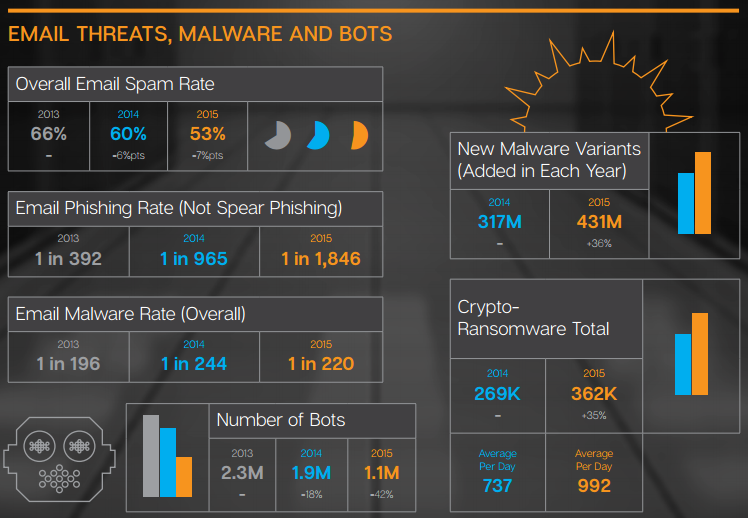
\includegraphics[width=1\textwidth]{malware-symantec}
	\caption{Infografía sobre el malware en 2016 \cite{malware-symantec}}
	\label{fig:malware-symantec}
\end{figure}

\subsection{Gusanos}

Una de las primeras categorías de malware que surge es la de los gusanos. Los gusanos (también conocidos como \textit{worms} por su término en inglés) son programas autorreplicantes que, en vez de infectar archivos concretos, se instalan directamente en los sistemas y buscan, mediante diferentes vulnerabilidades en los sistemas o técnicas como la ingeniería social, replicarse en la medida en la que les sea posible.

Fueron uno de los primeros tipos de malware y fueron una de las causas principales del desarrollo en los campos de la seguridad informática más defensiva. Un ejemplo es el famoso gusano \emph{ILOVEYOU} \cite{top-10-viruses}, el cual infectó en el año 2000 a decenas de millones de ordenadores con Windows. Otros también famosos son \emph{Code red}, \emph{Sasser} o \emph{Conficker}. Son uno de los tipos de malware que mayor daño económico han causado, causando daños estimados en miles de millones de euros en los casos mencionados.

Hoy en día, aunque siguen considerándose una amenaza, han quedado relegados a un segundo plano, por una parte, por la capacidad de los sistemas de firewall o sistemas antivirus de detectarlos y neutralizarlos y, por otra parte, por el surgimiento de otros tipos de malware, como los que se mencionan en los siguientes puntos.

\subsection{Troyanos}

Otro tipo de malware famoso son los troyanos. El nombre de troyano proviene del caballo de Troya, una gran estructura de madera que usó el pueblo griego en la guerra de Troya para introducir a sus soldados en la ciudad, que estaba completamente fortificada. De la misma manera, el malware denominado troyano se camufla, es decir, se oculta como un programa legítimo imitando el comportamiento de dicho programa, cuando en realidad son una forma para dar acceso a un atacante a los recursos de dicho sistema. Uno de los troyanos mas famosos fue \emph{Zeus} \cite{top-10-viruses}, que llego a infectar a más de un millón de ordenadores. También existe otros como, por ejemplo, \emph{CryptoLocker}, que es una mezcla entre troyano y ransomware, tipo de malware que se explica a continuación.

\subsection{Ransomware}

Según McAfee Labs \cite{mcafee-predictions} (actualmente parte de Intel) el ransomware es una de las mayores amenazas a día de hoy. El ransomware es un tipo de malware informático que busca beneficio económico en base a la extorsión hacia los usuarios. Para ello este clase de malware cifra los archivos de los usuarios para que sean inaccesibles para ellos, de tal manera que solo mediante el pago de cierta cantidad económica puedan recuperar dichos archivos.

Existen varias familias de ransomware, entre los que destacan \emph{CryptoWall 3}, \emph{CTB-Locker} o \emph{CryptoLocker}. El concepto de familias proviene de que en su mayoría se trata del mismo malware con prácticamente el mismo funcionamiento, pero con ligeras variaciones es su código que les permite eludir las posibles medidas de seguridad. En la figura \ref{fig:ransomware} se puede observar su crecimiento durante estos últimos años.

\begin{figure}[H]
	\centering
	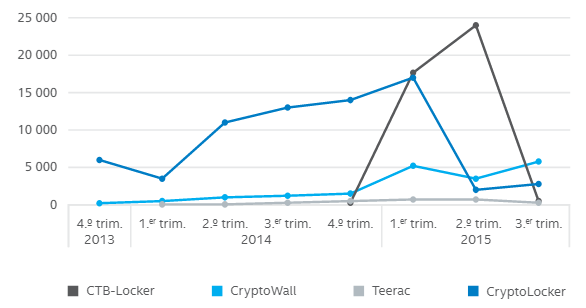
\includegraphics{ransomware}
	\caption{Nuevas muestras de familias de ransomware prominentes \cite{mcafee-predictions}}
	\label{fig:ransomware}
\end{figure}

Podemos encontrar incluso ejemplos relativamente recientes como puede ser \textit{WannaCry}, ransomware que afecto hace no mucho a decenas de países inutilizando sistemas de diversa índole, desde la Intranet de Telefónica hasta varios hospitales en Reino Unido \cite{wannacry1} \cite{wannacry2}.


\subsection{Rootkits}

Los rootkits son una clase de malware que tiene como objetivo principal escalar privilegios en el sistema, también conocido como conseguir acceso de superusuario o \textit{root}. No hace falta mencionar que con dichos privilegios el daño que puede causar en un sistema es inconmensurable, pudiendo dejarlo completamente inutilizado o eliminar absolutamente toda su información.

\subsection{RATs}

Los \textit{Remote Administration Tools} también conocidos como RAT, buscan ofrecer a los posibles atacantes una puerta trasera para acceder a los sistemas para así poder introducir otros tipos de malware específicos.

\subsection{Spyware}

Un tipo de malware concreto bastante popular desde la década del 2000 es el denominado spyware, cuyo objetivo es obtener información de las acciones de un sistema, infectando la máquina destino de manera inadvertida para el usuario, el cual desconoce que su actividad y/o sus datos están siendo monitorizados.

\subsection{Keyloggers}

El \textit{Keystroke Logger}, mejor conocido como Keylogger, es otro tipo de malware usado actualmente debido a su efectividad cuyo objetivo consiste en obtener la información de las pulsaciones que se realizan en un teclado de un sistema concreto. Este mecanismo tiene como principal objetivo extraer información, especialmente contraseñas, de un usuario para después poder acceder a los servicios que usa dicho usuario. Se puede encontrar Keyloggers tanto a nivel físico, en forma de pequeños dispositivos\footnote{\url{https://www.keelog.com/}} USB con una memoria interna\footnote{\url{https://store.hackaday.com/products/usb-rubber-ducky-deluxe}}, como a nivel de software, estos últimos especialmente sencillos de implementar con solo unas pocas lineas de código \cite{ander-keylogger}.

%------------------------------------------------------------------------------

\section{Dispositivos móviles}

El malware afecta a los sistemas y es un riesgo para la seguridad de estos, pero no es el único. Además hay que tener en cuenta que en los últimos años el mundo de las tecnologías de la información ha sufrido cambios drásticos. Ya no tenemos el modelo clásico de ordenadores personales y servidores estándar que conforman Internet. Han entrado a la palestra nuevas áreas que se han ido desarrollando. A medida que estas áreas han ido destacando, el campo de la seguridad informática ha ido avanzando para satisfacer las necesidades de seguridad de estas áreas y adaptarse a ellas mediante nuevas técnicas y medidas de seguridad.

Una de las áreas que ha destacado estos últimos años es el área de la seguridad de dispositivos móviles. Datos como que el consumo de Internet a día de hoy es mayor en este tipo de dispositivos que en ordenadores convencionales resultan sorprendentes. En el caso concreto de España, del 78,7\% de la población que se conecta regularmente a Internet, el 88,3\% de los usuarios lo hace a través de un smartphone \cite{smartphones-internet}. Teniendo eso en cuenta, es lógico que la seguridad estos dispositivos sea una prioridad y a su vez uno de los puntos de enfoque por parte de todo tipo de atacantes.

Los smartphones tienen una gran cantidad de usos diferentes. Aparte de ser la principal herramienta de comunicación, también son dispositivos mediante los que se procesa una gran cantidad de información, desde información personal como fotos o mensajes a información relacionada con el ámbito empresarial como documentos o correos. Debido a que la información ya no solo se procesa y transmite desde ordenadores tradicionales, sino que en su mayoría se hace desde dispositivos móviles, resulta necesario definir e implantar técnicas y procedimientos de seguridad en este tipo de dispositivos.

\subsection{Seguridad en smartphones}

Aunque en esencia los smartphones se traten de dispositivos basados en Linux, Unix o derivados, este tipo de dispositivos tienen sus particularidades con respecto a los ordenadores personales. Primeramente, estos sistemas no disponen de la arquitectura x86/x86-64 (al menos en su gran mayoría), sino que se basan en procesadores con arquitectura ARM. Debido a esto y al enfoque de uso que tienen, usan diferentes sistemas operativos que distan de los tradicionales. Los sistemas operativos más usados para smartphones son Android e iOS, que se encuentran en un 86,22\% y 12,88\% de los dispositivos vendidos en 2016 \cite{gartner-uso-so}, respectivamente.

Ambos son sistemas que, al estar por defecto más limitados en uso y configuración, resultan \textit{a priori} más seguros que los sistemas operativos de escritorio. Existen una serie de técnicas que se suelen aplicar independientemente del sistema operativo utilizado, como pueden ser la firma de aplicaciones o el uso de cifrado para ciertos casos. Aun así, este tipo de medidas son prácticamente obligatorias para disponer de sistemas mínimamente seguros. Lo que diferencia a cada uno de los sistemas operativos desde el punto de vista de la seguridad es tanto el enfoque de seguridad que le dan al sistema como las técnicas, medidas, arquitecturas de software o algoritmos, que cambian de un sistema operativo a otro.

\subsubsection{Seguridad en iOS}

En dispositivos con iOS la seguridad se enfoca desde varios puntos. Uno de los puntos en los que iOS destaca es en su tienda de aplicaciones, que dispone de ciertos filtros y controles de seguridad a la hora de publicar aplicaciones para dificultar en la mayor medida posible que a través de las aplicaciones entre algún tipo de malware.

Por otro lado, uno de los puntos más fuertes de iOS es el relacionado con en el cifrado. Debido a la ventaja que otorga el hecho de que la misma compañía elabore tanto el hardware como las diferentes capas de software de sus dispositivos, se pueden integrar medidas de seguridad en el propio hardware que funcionen de manera conjunta a su software. Una de las más destacables es la incorporación del coprocesador llamado \emph{Secure Enclave} \cite{ios-sec-guide}. Este coprocesador (disponible en el Apple S2, y en el Apple A7 y posteriores) se encarga de todas las operaciones criptográficas para la gestión de claves de cifrado de datos y mantiene la integridad de la protección de datos, incluso si el kernel del sistema se ha visto comprometido. Usa memoria cifrada e incluye un generador aleatorio de números por hardware. La comunicación entre este coprocesador y el procesador principal esta completamente aislada del resto del sistema.

Esto tiene dos ventajas. La primera, que el cifrado por hardware, al realizarse de manera transparente a cualquier capa de software, resulta díficilmente evitable. Por otra parte, a nivel de rendimiento, resulta mucho más eficiente que cualquier tipo de cifrado por software.

Además, todos los dispositivos iOS tienen un sistema de cifrado mediante hardware y AES-256 que se sitúa entre la memoria principal y el almacenamiento flash \cite{ios-sec-guide}, de tal manera que los datos almacenados en los dispositivos se mantienen cifrados sin que se pierda rendimiento en ello. Para cada sistema de cifrado se crea identificadores únicos tanto par cada usuario (UID) como para cada grupo distinto de dispositivos (GID), ambos integrados en el propio hardware. Cada UID es único y no es conocido ni por Apple ni por ninguna aplicación ni usuario. Cada GID es común a una familia de dispositivos y se usa para distinguirlos entre sí. Esto hace que los datos que se almacenan sean altamente difíciles de descifrar.

Las operaciones de cifrado y descifrado concretas siguen el esquema que se muestra en la Figura \ref{fig:ios-data-encrypt} , haciendo uso también de una contraseña propia elegida por el usuario, la que se muestra en el diagrama con el nombre de \textit{Passcode Key}.

\begin{figure}[H]
	\centering
	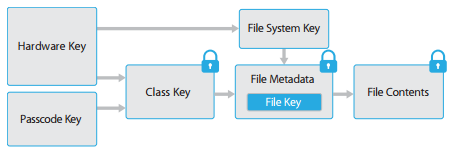
\includegraphics{ios-data-encrypt}
	\caption{Esquema de cifrado de un archivo en iOS}
	\label{fig:ios-data-encrypt}
\end{figure}

\subsubsection{Seguridad en Android}

El modelo de seguridad en Android se diferencia del modelo de iOS en varios aspectos. Más que en un fuerte cifrado a todos los niveles, el cual también usa pero en menor medida, el enfoque se basa en hacer lo más segura posible cada aplicación. Esto es lógico teniendo en cuenta que, por un lado, la tienda de aplicaciones de Android, la Play Store\footnote{\url{https://play.google.com/store/apps}}, es menos estricta que la de iOS y que, por otro lado, Google (propietaria de Android) no fabrica los dispositivos que integran dicho sistema. Por ello, la arquitectura de software del sistema resulta más jerárquica, y es fundamental para las diversas medidas de seguridad que se implementan. En la Figura \ref{fig:android-arch} se muestran las diferentes capas de dicha arquitectura. 

\begin{figure}[H]
	\centering
	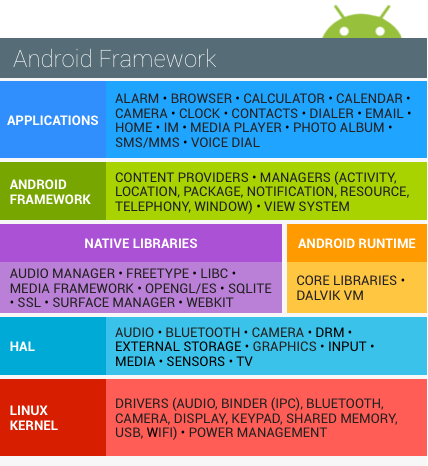
\includegraphics{android-arch}
	\caption{Las diferentes capas que componen la arquitectura de Android}
	\label{fig:android-arch}
\end{figure}

La esencia de la seguridad en Android reside en controlar y limitar la interacción entre las diferentes capas para evitar fallos de seguridad. Para ello se hace uso de diferentes técnicas \cite{android-sec-guide} \cite{jspdcp-2014}:

\begin{itemize}
	\item El \emph{sandboxing}, donde el código de cada aplicación se ejecuta de manera aislada al resto de aplicaciones y, además, los datos de cada aplicación se mantienen separados \cite{jspdcp-2014}. 
	\item Un framework de aplicaciones que implementa ciertas técnicas comunes de seguridad como, por ejemplo, métodos criptográficos, sistemas de permisos o una comunicación entre procesos (\textit{IPC, Interprocess Communication}) segura.	
	\item Implementar diversas tecnologías como ASLR (\textit{Address Space Layout Randomization}), NX (\textit{No-eXecute}), \textit{ProPolice}, \textit{safe\textunderscore iop, OpenBSD dlmalloc}, \textit{OpenBSD calloc}, y \textit{Linux mmap\textunderscore min\textunderscore addr} para evitar errores de \textit{buffer overflow}, para evitar que se ejecuten instrucciones concretas o para mitigar otro tipo de riesgos relacionados con la gestión de la memoria.
	\item Un sistema de cifrado de archivos mediante AES-256 para proteger los datos almacenados en los dispositivos.
	\item Un sistema de permisos tanto a nivel de usuario como al nivel de cada aplicación concreta para controlar las acciones de los usuarios y las aplicaciones.
\end{itemize}

Ente enfoque hace que, por una parte, el propio Android mediante su arquitectura y el uso de una VM (Virtual Machine) específicamente creada para el sistema (como se puede observar en la Figura \ref{fig:android-arch}) ofrezca un repertorio de mecanismos de seguridad que hacen de él un sistema relativamente seguro. Por otra parte, también pone empeño en que los desarrolladores tienen la necesidad de implementar medidas de seguridad en sus aplicaciones para garantizar la seguridad de las mismas. Para ello, el SDK de Android proporciona acceso a un gran número de utilidades como, entre otras, utilidades de cifrado, de manejo de credenciales o de intercambio de mensajes.

%------------------------------------------------------------------------------

\section{Internet of Things}

También junto a la seguridad de los dispositivos móviles, que viene determinada por el auge de dichos dispositivos, el área de la seguridad del Internet of Things (conocida como IoT) es una de las áreas que más impulso está teniendo, debido al mismo motivo. Cada vez hay una mayor cantidad de dispositivos conectados a Internet, que no ha hecho más que crecer exponencialmente debido al IoT. Dispositivos que ya no se tratan solo de móviles, tablets u ordenadores, sino de otro tipo de dispositivos, como electrodomésticos, que han sido dotados de capacidad de computación y conexión a Internet para ampliar sus capacidades y poder recopilar información de ellos. En esencia, el IoT se basa en una serie de dispositivos a los que, mediante el uso de sensores, procesadores y conexión a Internet, se les da la capacidad de recoger y transmitir información a otros dispositivos, además de recibir dicha información para actuar de una manera u otra.

\subsection{Aplicaciones}

Las aplicaciones de lo que se denomina Internet of Things son amplísimas. Prácticamente cualquier sistema electrónico que disponga de una serie de sensores mediante los cuales obtiene información puede ver multiplicadas sus capacidades añadiéndole una conexión a la red. De esta manera se le dota de capacidad para ya no solo transmitir información sino incluso poder interactuar de forma más compleja con otra serie de sistemas \cite{Miorandi20121497} \cite{Gubbi20131645}.
	
\subsubsection{Smart homes}

Mediante tecnologías IoT se puede dotar a los diferentes elementos domóticos de un hogar o edificio de capacidades para reaccionar de manera automática a diferentes cambios que se puedan dar. Desde controlar la luz o el agua hasta controlar la temperatura o las persianas, todo de tal manera que los subsistemas sean capaces de comunicarse y actuar de manera conjunta en función de la información que reciben.
	
\subsubsection{Smart Cities}

El término Smart Cities se refiere al sistema ciberfísico que conforma una red avanzada de comunicación para optimizar el uso de los sistemas físicos de una ciudad. Puede optimizar servicios como por ejemplo el tendido eléctrico, mediante el análisis de consumo de toda la red eléctrica, o la red de carreteras, mediante sistemas avanzados de control de tráfico (del cual los vehículos autónomos se pueden beneficiar). Esos son solo unos breves ejemplos de lo que un sistema de este tipo puede llegar a optimizar dentro de los procesos que se dan en una ciudad.
	
\subsubsection{Monitorización medioambiental}

El IoT también puede servir para monitorizar cambios en el medio ambiente e integrar todo esa adquisición de datos para que funcione de manera conjunta con otros sistemas. Una serie de sistemas de tiempo real, a los que se añade la capacidad de comunicarse e interactuar entre sí, pueden ser una plataforma sólida mediante la cual detectar y monitorizar anomalías que afecten a la vida humana, animal y vegetal. Además, pueden ser una herramienta fundamental para obtener información que permita mitigar los efectos de cualquier tipo de contaminación medioambiental.
	
\subsubsection{Sanidad}

La sanidad también es uno de esos sectores que se puede beneficiar de los avances en el IoT. Por ejemplo, la capacidad para monitorizar diferentes parámetros (como la temperatura corporal, la presión sanguínea o la actividad cardíaca) de manera constante puede ser una herramienta fundamental a la hora de prevenir y tratar diversas enfermedades. Además del nivel patológico, se puede usar  diferentes dispositivos para tomar información que permita mejorar el estilo de vida y la salud de las personas. Dispositivos como los wearables son un buen ejemplo de ello, entre los que se encuentran las famosas pulseras cuantificadoras. 
	
\subsubsection{Smart Business}

El término Smart Business hace referencia a todas esas aplicaciones del Internet of Things que se usan para mejorar tanto la logística interna como los productos y servicios que ofrece una empresa o negocio. La gestión de inventario tiempo real o la automatización del envío de información sobre productos para ofrecer un mejor servicio post venta son dos ejemplos en los que enfatizan cada vez mas empresas.
	
\subsubsection{Seguridad y vigilancia}

Aunque pueda ser polémico, el Internet of Things también se puede aplicar en el área de la seguridad y vigilancia. Los sistemas interconectados de cámaras o los sensores para detectar químicos nocivos son dos ejemplos. El primero de ellos no se respeta la privacidad del usuario, mientras que el segundo sí. Debido a eso, aplicaciones como la primera son objeto de numerosas críticas por parte de diversas organizaciones.

\subsection{Seguridad en Internet of Things}

Uno de los principales problemas del Internet of Things reside en que ya no solo se trata de el peligro de que la información se vea comprometida o revelada sino que, al tratarse de otra serie de dispositivos, los peligros son mucho mayores \cite{iot-qz}\cite{iot-techradar}. Esto es algo de lo que el mundo de la seguridad informática ya se ha percatado. Estimando que el numero de dispositivos conectados a Internet pasará de 6,4 mil millones en 2016 a 21 mil millones en 2020 \cite{iot-searchdatacenter} debido al auge del IoT, resulta fundamental indagar en ello. 

En la actualidad existen gran cantidad de casos en los que diferentes dispositivos salen al mercado con esas capacidades para conectarse a Internet pero que carecen de prácticamente ningún tipo de medida de seguridad. Se han dado casos como el de Miele \cite{iot-miele} donde a causa de la falta de seguridad en un modelo de sus lavavajillas, se puede llegar a acceder a la red local privada a donde este conectado de manera sencilla. Otro caso es el de los automóviles Tesla \cite{iot-tesla}, donde más de una vez se han descubierto vulnerabilidades que permiten obtener el control total de sus vehículos y conducirlos remotamente a placer del atacante. Esto es gravísimo, pudiendo llegar a poner en en riesgo la vida de personas. Por ello, los servicios de la seguridad informática son mas necesarios si cabe para este campo. 

%------------------------------------------------------------------------------

\section{Cloud Computing}

El Instituto Nacional de Estándares y Tecnologías de Estados Unidos, conocido como NIST (\textit{National Institute of Standards and Technologies}) define el Cloud Computing como:

\begin{quotation}
\textit{''Un modelo para hacer posible el acceso a red adecuado y bajo demanda a un conjunto de recursos de computación configurables y compartidos (por ejemplo, redes, servidores, almacenamiento, aplicaciones y servicios…) cuyo aprovisionamiento y liberación puede realizarse con rapidez y con un mínimo esfuerzo de gestión e interacción por parte del proveedor de dicha nube''.} \cite{inteco-cloud}
\end{quotation}

Podemos entender como Cloud Computing a una extensión de las aplicaciones de Internet, que eran principalmente aplicaciones web y transmisión de datos, a nuevas posibilidades, entre las cuales se incluyen plataformas completas y software más complejo, ofrecidas como un modelo de servicio configurable y escalable.

Las estructuras cloud se pueden clasificar en tres categorías: públicas, comunitarias y privadas. En las primeras el acceso a sus servicios es abierto, mientras que en las segundas está acotado a un determinado entorno, normalmente una empresa. En la última, aunque no se tiene acceso público a sus servicios, estos se comparten entre varias entidades.

\subsection{Tipos de servicios}

El Cloud Computing puede ofrecer una serie de servicios a sus usuarios, y en función de qué servicio se ofrezca, se clasifica en una de las tres categorías diferentes existentes que se mencionan a continuación.

\subsubsection{Software as a Service}

\emph{Software as a Service} consiste en un despliegue de software en el cual las aplicaciones y los recursos computacionales se han diseñado para ser ofrecidos como servicios de funcionamiento bajo demanda. De esta forma se reducen los costes tanto de software como hardware, así como los gastos de mantenimiento y operación. En esta categoría las consideraciones sobre seguridad son responsabilidad del proveedor del servicio, estando limitada la configuración que puede realizar el suscriptor.

\subsubsection{Platform as a Service}

\emph{Platform as a Service} es el servicio donde se ofrece una plataforma en la cual el suscriptor del servicio puede desplegar su propio software. Con ello se reducen los costes y la complejidad de la compra, el mantenimiento, el almacenamiento y el control del hardware y el software que componen la plataforma. El suscriptor del servicio tiene control parcial sobre las aplicaciones y la configuración del entorno ya que la instalación de los entornos dependerá de la infraestructura que el proveedor del servicio haya desplegado. La seguridad se comparte entre el proveedor del servicio y el suscriptor ya que el suscriptor aporta su propio software.

\subsubsection{Infrastructure as a Service}

\emph{Infrastructure as a Service} es un modelo en el cual la infraestructura (servidores, software y equipamiento de red) es gestionada por el proveedor como un servicio bajo demanda, en el cual se pueden crear entornos para desarrollar, ejecutar o probar aplicaciones, El fin principal de este modelo es evitar la compra de recursos por parte de los suscriptores, ya que el proveedor ofrece estos recursos como objetos virtuales accesibles a través de un interfaz de servicio. El suscriptor mantiene generalmente la capacidad de decisión del sistema operativo y del entorno que instala. Por lo tanto, la gestión de la seguridad corre principalmente a cargo del suscriptor.

\subsection{Seguridad en Cloud Computing}

Debido al auge del Cloud Computing surge la CSA (\textit{Cloud Security Alliance}). La CSA se define como una organización internacional sin ánimo de lucro que tiene como objetivo promover el uso de una serie de buenas prácticas para garantizar la seguridad en la nube.
Entre otras actividades, la CSA elabora un informe periódico con las mayores amenazas de seguridad de sistemas de Cloud Computing \cite{csa-cloud-12-threats}. Estas amenazas se actualizan regularmente buscando el consenso de los expertos. A continuación, se resumen las amenazas descritas en este informe. En el informe de 2016, la CSA marca como amenazas más graves, ordenadas por orden de importancia, los siguientes 12 puntos:
\begin{enumerate}
	\item Brechas de Datos
	\item Manejo inseguro de Credenciales de Acceso
	\item Interfaces y APIs inseguros
	\item Vulnerabilidades de Sistemas y Aplicaciones
	\item Secuestro de Cuentas
	\item Amenazas Internas
	\item Advanced Persistent Threats (APTs)
	\item Pérdida de Datos
	\item Diligencia insuficiente
	\item Abuso y mal uso del Cloud Computing
	\item Denegación de Servicio
	\item Problemas derivados de las tecnologías compartidas
\end{enumerate}

Con el auge del Cloud Computing, este tipo de amenazas son cada vez más graves. Desde servicios de almacenamiento de datos hasta plataformas de despliegue de aplicaciones, cada vez más empresas y usuarios delegan almacenamiento, infraestructura, o software en servicios de Cloud Computing, por lo que, en primer lugar, ser conscientes de la ventajas, inconvenientes y, sobre todo, riesgos que acarrea el uso de estos servicios resulta fundamental para después, en segundo lugar, ser capaces de securizarlos en la mayor medida posible y hacer un uso seguro de esto servicios.